\documentclass[aspectratio=169,
				xcolor=table]{beamer}
				
% Load general definitions
\usepackage[utf8]{inputenc}
%\usepackage[T1]{fontenc}
\usepackage[brazil]{babel}
\usepackage{amsmath}
\usepackage{amsfonts}
\usepackage{amssymb}
\usepackage{graphicx}
\usepackage{verbatim}
\usepackage{cancel}
\usepackage{askmaps}
\usepackage{tabularx}
\usepackage[table]{xcolor}
%\usepackage{tikz}
\usepackage{multirow}
\usepackage{mathtools}
\usepackage{color, colortbl}
\usepackage{etoolbox}
\usepackage{pbox}
\usepackage{changepage}
\usepackage{xpatch}
\usepackage{array}
\usepackage{marvosym}
\usepackage{tabu}
\usepackage{multicol}
\usepackage{listings}
\usepackage{underscore}
\usepackage{filecontents}
\usepackage[]{algorithm2e}
\usepackage{ragged2e}

\newcolumntype{P}[1]{>{\centering\arraybackslash}m{#1}}
\definecolor{Gray}{gray}{0.75}
\definecolor{Gray2}{gray}{0.85}

\definecolor{lightBlue}{HTML}{DAE8FC}
\definecolor{Blue}{RGB}{51, 51, 204}

%\useinnertheme[lily]{rounded}
\usetheme{UniEvangelica}
%\usetheme{Copenhagen}
%\usetheme{Berlin}
%\usecolortheme{dolphin}
\tolerance=1
\emergencystretch=\maxdimen
\hyphenpenalty=10000
\hbadness=10000

\setbeamertemplate{navigation symbols}{}%remove navigation symbols


\let\olditem=\item% 
\renewcommand{\item}{\olditem \justifying}%
\def\center{\trivlist \centering\item\relax}
\def\endcenter{\endtrivlist}

\setbeamertemplate{itemize/enumerate body begin}{\large}
\setbeamertemplate{itemize/enumerate subbody begin}{\large}

\setbeamertemplate{itemize item}{\raisebox{0.1ex}{$\blacktriangleright$}\hskip0.1em}
\setbeamertemplate{itemize subitem}{\raisebox{0.1ex}{$\blacktriangleright$}\hskip0.1em}

\newcommand{\greenarrow}{\textcolor{green}{\rotatebox[origin=c]{180}{\MVArrowDown}}}

\newcommand{\redarrow}{\textcolor{red}{\MVArrowDown}}

%\newcommand{\ftable}{
%	\begin{table}
%		\large
%		\centering
%		\rowcolors{1}{\ifnumless{\rownum}{2}{Blue}{lightBlue}}{}
%}

\newenvironment{eftable}{
	\begin{table}
		\large
		\centering
		\rowcolors{1}{}{Blue}
		\rowcolors{1}{\ifnumless{\rownum}{2}{Blue}{lightBlue}}{}
	}
	{
	\end{table}
}


%\setbeamertemplate{frametitle}
%{
%	%\vspace*{-2em}	
%	\insertframetitle
%
%	 %\textcolor{white}{\LARGE \insertframetitle}
%
%}

% Specific definitions
\title[]{Arquitetura e Organização de Computadores}
\subtitle[]{Unidade Central de Processamento - Parte 2}
\author[]{Prof. Alexandre Tannus}
\date{}

%\AtBeginSection{\frame{\sectionpage}}

\begin{document}

	\begin{frame}
		\titlepage
	\end{frame}

	\begin{frame}
		\tableofcontents		
	\end{frame}	
		
	\section{Instruções}

	\begin{frame}
		\frametitle{Conjunto de Instruções}
		\begin{itemize}
			\item Interface entre o programador e a máquina
			\vspace{1em}
			\item Cada instrução realiza uma tarefa simples
			\vspace{1em}
			\item Operações complexas podem ser construídas a partir de operações simples
		\end{itemize}
	\end{frame}
	
%	\begin{frame}
%		\frametitle{Exemplo}
%		\begin{lstlisting}
%add		$t8, $s2, $s3
%add		$t9, $s5, $s6
%add		$s7, $t8, $t9
%		\end{lstlisting}
%	\end{frame}	
	
	\begin{frame}
		\frametitle{Formato das instruções}
		\begin{itemize}
			\item Execução sequencial
			\vspace{1em}
			\item Exceções
			\begin{itemize}
				\item Instruções de salto
				\item Instruções de desvio
			\end{itemize}
		\end{itemize}
	\end{frame}
	
	\begin{frame}
		\frametitle{Tipos de instruções}
		\begin{eftable}
		\Large
		\resizebox{\textwidth}{!}{
		\begin{tabular}{@{}  c | m{3cm} | m{2.5cm} | m{2.5cm} | m{2.5cm} | m{2.5cm} | m{3cm} @{}}
			
			\textcolor{white}{Tipo} &
			\multicolumn{6}{|c|}{\textcolor{white}{Formato (bits)}} \\
			
			R & opcode (6) & rs(5) & rt(5) & rd(5) & shamt(5) & function(6) \\
			
			I & opcode (6) & rs(5) & rt(5) & \multicolumn{3}{|c|}{imediato(16)} \\
			
			J & opcode(6) & \multicolumn{5}{|c|}{endereço(26)} \\
			
		\end{tabular}}
		\end{eftable}
	\end{frame}
	
	\begin{frame}
		\frametitle{Instruções Aritméticas e Lógicas Básicas}
		
		\begin{eftable}
			\begin{tabular}{c |c |l | c}
			 \textcolor{white}{Operação} & 
			 \textcolor{white}{Comando} & 
			 \textcolor{white}{Sintaxe} &
			 \textcolor{white}{Função} \\
			 Adição & $add$ & $add \quad \$t0, \$s0, \$s1$ & 32\\
			 Subtração & $sub$ & $sub \quad \$t0, \$s0, \$s1$ & 34\\
			 Lógica AND & $and$ & $and \quad \$t0, \$s0, \$s1$ & 36\\
			 Lógica OR & $or$ & $or \quad \$t0, \$s0, \$s1$ & 37\\
			 Lógica XOR & $xor$ & $xor \quad \$t0, \$s0, \$s1$ & 38\\
			 Lógica NOR & $nor$ & $nor \quad \$t0, \$s0, \$s1$ & 39\\

			 Adição imediata& $addi$ & $addi \quad \$t0, \$s0, constante$ & 8\\	
			 Lógica AND imediata& $andi$ & $andi \quad \$t0, \$s0, constante$ & 12\\
			 Lógica OR imediata& $ori$ & $ori \quad \$t0, \$s0, constante$ & 13\\
			 Lógica XOR imediata& $xori$ & $xori \quad \$t0, \$s0, constante$ & 14\\

			\end{tabular}
		\end{eftable}
	\end{frame}

	\begin{frame}
		\frametitle{Instruções de Carga (\textit{Load)}e Armazenamento (\textit{Store)}}
		\begin{itemize}
			\item Transferência de 32 bits entre memória e registradores
			\vspace{1em}
			\item Instrução tipo I
			\vspace{1em}
			\item Regsitrador \textit{rt} - destino (\textit{load}) ou origem (\textit{store)}
			\vspace{1em}
			\item Endereço de memória - Constante de deslocamento + valor do registrador \textit{rs}
		\end{itemize}
	\end{frame}
	
	\begin{frame}
		\frametitle{Instruções de Salto (\textit{Jump)} e Desvio (\textit{Branch})}
		\begin{itemize}
			\item Alteram o fluxo de execução sequencial
			\vspace{1em}
			\item Salto
			\begin{itemize}
				\item Instrução \textit{j} ou \textit{jr}
			\end{itemize}
			\vspace{1em}
			\item Desvio
			\begin{itemize}
				\item \textit{bne} - diferente de
				\item \textit{bltz} - menor que
				\item \textit{beq} - igual a
			\end{itemize}
		\end{itemize}
	\end{frame}
	
	\begin{frame}
		\frametitle{Modos de endereçamento}
		\begin{itemize}
			\item Implícito
			\item Imediato
			\item Por registrador
			\item Base
			\item Relativo ao PC
			\item Pseudodireto
		\end{itemize}
	\end{frame}
	
	
	\begin{frame}
		\frametitle{Ciclo de Instrução}
		\begin{itemize}
			\item Busca
			\begin{itemize}
				\item Leitura da próxima instrução da memória
			\end{itemize}
			\vspace{1em}
			\item Execução
			\begin{itemize}
				\item Interpretação e efetuação da operação indicada
			\end{itemize}
			\vspace{1em}
			\item Interrupção
			\begin{itemize}
				\item Verificação de ocorrência de interrupção
			\end{itemize}
		\end{itemize}
	\end{frame}
	
	\begin{frame}
		\frametitle{Ciclo de instrução}
		\begin{figure}
			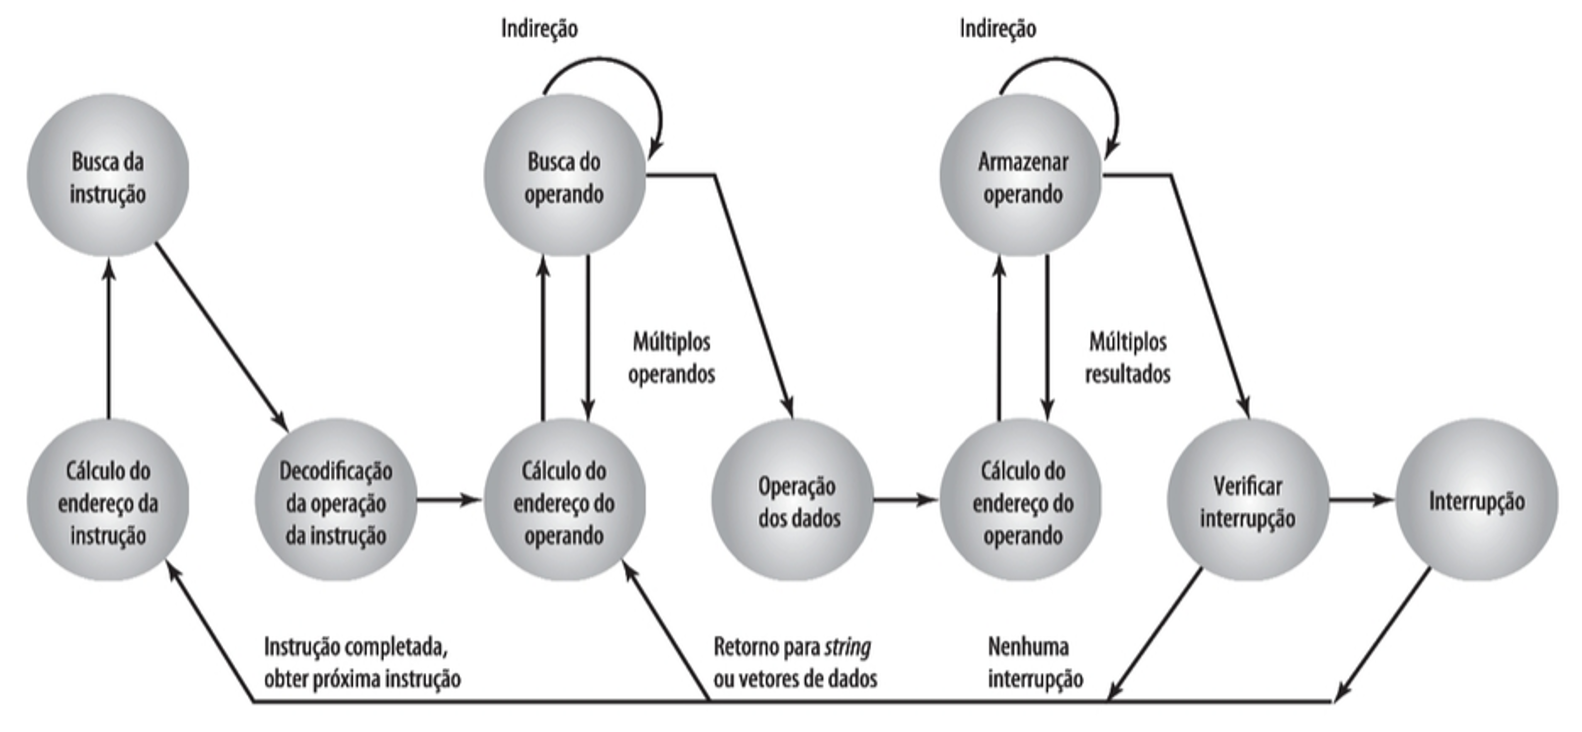
\includegraphics[height=0.8\textheight , keepaspectratio]{../figs/cap06/intrucao.png} 
		\end{figure}
	\end{frame}
	
	\begin{frame}
		\frametitle{Arquitetura CISC}
		\begin{itemize}
			\item Anos 80 – computadores mais complexos
			\vspace{1em}

			\item CISC – \textit{Complex Instruction Set Computer}
			\vspace{1em}

			\item Conjuntos de instruções cada vez mais complexas e maiores
			\begin{itemize}
				\item Pode afetar o desempenho
				\item Maior dificuldade de implementação de outras funções

			\end{itemize}

		\end{itemize}
	\end{frame}
	
	\begin{frame}
		\frametitle{Arquitetura RISC}
		\begin{itemize}
			\item RISC – \textit{Reduced Instruction Set Computer}
			\vspace{1em}

			\item Diminuição do número de instruções disponíveis
			\vspace{1em}
			
			\item Padronização do tamanho das instruções
			\vspace{1em}

			\item Introdução do pipeline
		\end{itemize}
	\end{frame}
	
	\begin{frame}
		\frametitle{Arquitetura RISC}
		\begin{itemize}
			\item Controle via \textit{hardware}
			\vspace{1em}
			\item Maior número de registradores
			\vspace{1em}
			\item Modos de endereçamento limitados
		\end{itemize}
	\end{frame}
	
	\section{Paralelismo}	
	
	\begin{frame}
		\frametitle{Paralelismo}
		\begin{itemize}
			\item Realizar várias coisas ao mesmo tempo
			\vspace{1em}	
			\item Dois níveis
			\begin{itemize}
				\item Instrução
				\item Processador
			\end{itemize}

		\end{itemize}
	\end{frame}
	
	\begin{frame}
		\frametitle{Paralelismo de instrução}
		\begin{itemize}
			\item Executar mais instruções em um determinado tempo
			\vspace{1em}
			\item Dois modelos
			\begin{itemize}
				\item \textit{Pipelines}
				\item Superescalares
			\end{itemize}

		\end{itemize}
	\end{frame}
	
	\begin{frame}
		\frametitle{\textit{Pipeline}}
		\begin{itemize}
			\item Dividir uma instrução em vários estágios

			\item Dedicar uma parte do \textit{hardware} para cada estágio

			\item Executar paralelamente vários estágios 

		\end{itemize}
	\end{frame}

	\begin{frame}
		\frametitle{\textit{Pipeline} de 6 estágios}
		\begin{figure}
			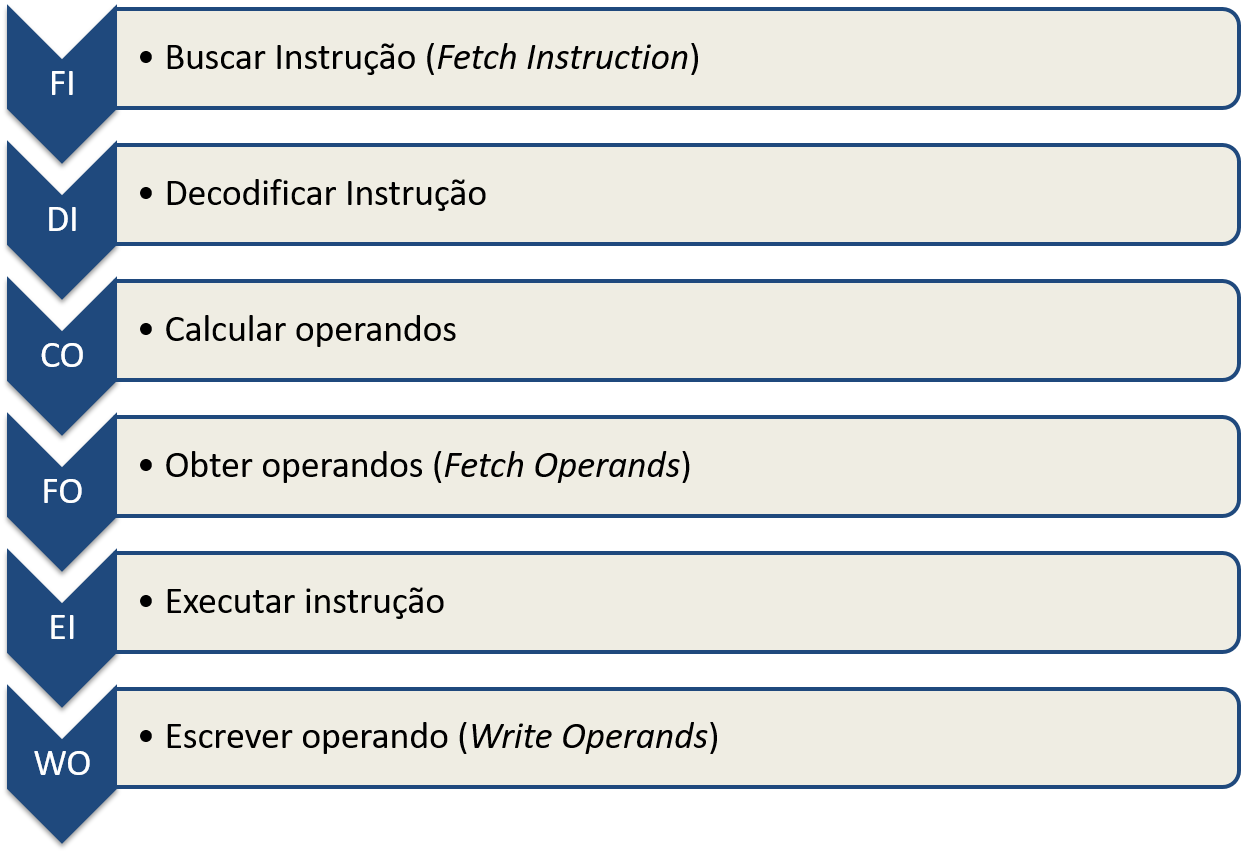
\includegraphics[height=0.8\textheight , keepaspectratio]{../figs/cap06/pipeline01.png} 
		\end{figure}
	\end{frame}
	
	\begin{frame}
		\frametitle{\textit{Pipeline} de 6 estágios}
		\begin{itemize}
			\item Buscar Instrução (Fetch Instruction)
			\begin{itemize}
				\item Leitura da próxima instrução 
			\end{itemize}
			\vspace{1em}
			\item Decodificar Instrução
			\vspace{1em}
			\item Calcular operandos
			\begin{itemize}
				\item Cálculo do endereço efetivo de cada operando
			\end{itemize}

		\end{itemize}
	\end{frame}

	\begin{frame}
		\frametitle{\textit{Pipeline} de 6 estágios}
		\begin{itemize}
			\item Obter operandos (Fetch Operands)
			\begin{itemize}
				\item Obtenção dos operandos da memória
			\end{itemize}
			\vspace{1em}
			\item Executar Instrução
			\begin{itemize}
				\item Realização da operação e armazenamento do resultado no registrador
			\end{itemize}
			\vspace{1em}
			\item Escrever operandos (\textit{Write Operands})
			\begin{itemize}
				\item Cálculo do endereço efetivo de cada operando
			\end{itemize}

		\end{itemize}
	\end{frame}
	
	\begin{frame}
		\frametitle{Executando instruções}

		\begin{eftable}
		\resizebox{\textwidth}{!}{
			\begin{tabular}{@{} l *{18}{c} @{}}
	            & 
	            \textcolor{white}{1}  & \textcolor{white}{2}  & 
	            \textcolor{white}{3}  & \textcolor{white}{4}  & 
	            \textcolor{white}{5}  & \textcolor{white}{6}  & 
	            \textcolor{white}{7}  & \textcolor{white}{8}  & 
	            \textcolor{white}{9}  & \textcolor{white}{10} & 
	            \textcolor{white}{11} & \textcolor{white}{12} & 
	            \textcolor{white}{13} & \textcolor{white}{14} & 
	            \textcolor{white}{15} & \textcolor{white}{16} & 
	            \textcolor{white}{17} & \textcolor{white}{18} \\
				Instrução 1 & FI & BI & CO & FO & EI & W0 &    &    &    &    &    &    &    &    &    &    &    &    \\
				Instrução 2 &    &    &    &    &    &    & FI & BI & CO & FO & EI & WO &    &    &    &    &    &    \\
				Instrução 3 &    &    &    &    &    &    &    &    &    &    &    &    & FI & BI & CO & FO & EI & WO
			\end{tabular}}
		\end{eftable}
	\end{frame}

	\begin{frame}
		\frametitle{Executando instruções}

		\begin{eftable}
		\resizebox{\textwidth}{!}{
			\begin{tabular}{@{} l *{18}{c} @{}}
	            & 
	            \textcolor{white}{1}  & \textcolor{white}{2}  & 
	            \textcolor{white}{3}  & \textcolor{white}{4}  & 
	            \textcolor{white}{5}  & \textcolor{white}{6}  & 
	            \textcolor{white}{7}  & \textcolor{white}{8}  & 
	            \textcolor{white}{9}  & \textcolor{white}{10} & 
	            \textcolor{white}{11} & \textcolor{white}{12} & 
	            \textcolor{white}{13} & \textcolor{white}{14} & 
	            \textcolor{white}{15} & \textcolor{white}{16} & 
	            \textcolor{white}{17} & \textcolor{white}{18} \\
								
				Instrução 1 & FI & BI & CO & FO & EI & W0 &    &    &   &    &    &    &    &    &    &    &    &    \\
				Instrução 2 &    & FI & BI & CO & FO & EI & WO &    &   &    &    &    &    &    &    &    &    &    \\
				Instrução 3 &    &    & FI & BI & CO & FO & EI & WO &   &    &    &    &    &    &    &    &    &   
			\end{tabular}}
		\end{eftable}
	\end{frame}
	
	\begin{frame}
		\frametitle{Superescalares}
		\begin{itemize}
			\item Execução de vários \textit{pipelines} simultaneamente

		\end{itemize}
		\begin{figure}
			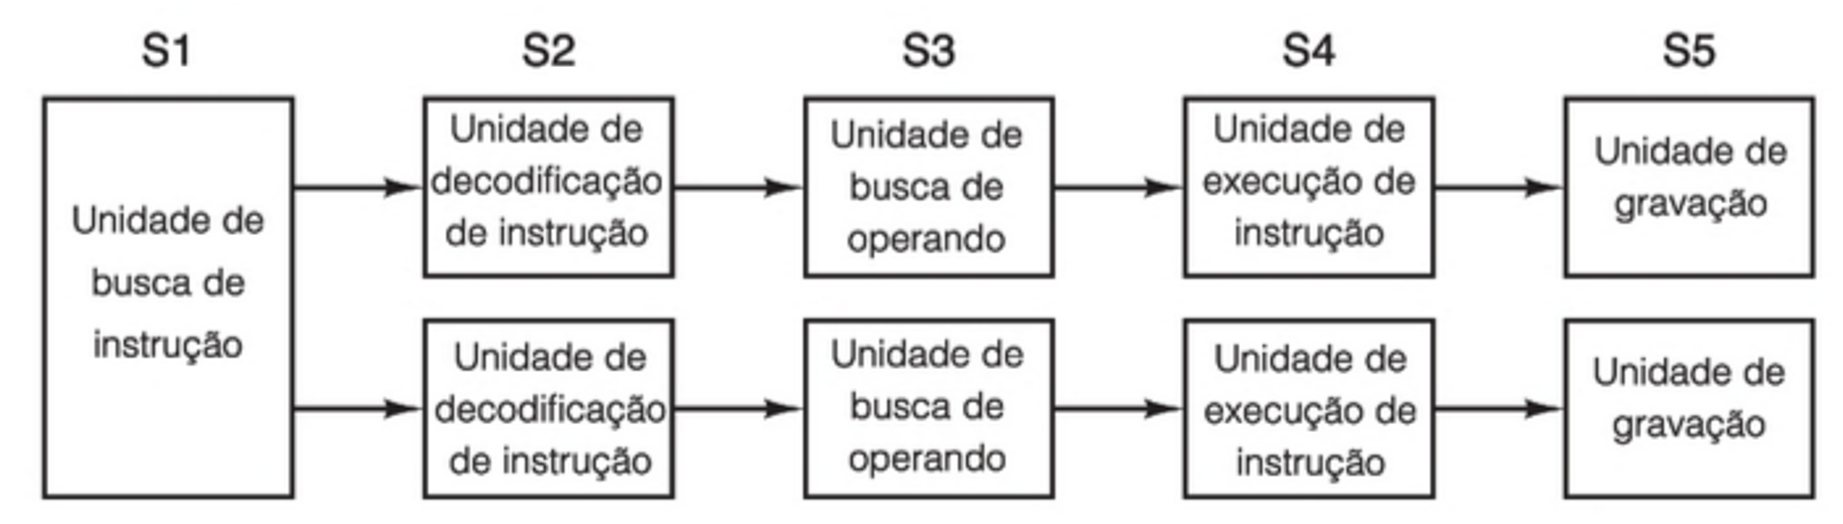
\includegraphics[width=\textwidth , keepaspectratio]{../figs/cap06/pipeline02.png} 
		\end{figure}
	\end{frame}	

	\begin{frame}
		\frametitle{Paralelismo de processador}
		\begin{itemize}
			\item Projeto de computadores com várias CPUs
			\vspace{1em}
			\item Modelos
			\begin{itemize}
				\item Computadores paralelos
				\item Multiprocessadores
				\item Multicomputadores

			\end{itemize}

		\end{itemize}
	\end{frame}
	
	\section{Unidade de Controle}		
		\begin{frame}
			\frametitle{CPU - Unidade de Controle}
			\begin{itemize}
				\item Controla toda a operação do microprocessador
				\vspace{1em}
				\item Constituída por
				\begin{itemize}
					\item Circuito de temporização
					\item Controle e decodificação
					\item Decodificador de instruções
				\end{itemize}
			\end{itemize}
		\end{frame}
	
	\section{Exercícios}	

	\begin{frame}
		\frametitle{}
		Dentro do conceito de organização de computadores, a UCP (Unidade Central de Processamento) desempenha um papel fundamental, sendo composta por diversas partes. Em particular, a Unidade de Controle é a parte da UCP responsável por
		\vspace{1em}
		\begin{enumerate}[a]
			\normalsize
			\item armazenar resultados temporários.
			\item indicar a próxima instrução a ser buscada na memória, para execução.
			\item buscar instruções na memória principal e determinar o tipo dessas instruções.
			\item armazenar o código da instrução que está sendo correntemente executado.
			\item realizar operações como adição e subtração sobre os valores presentes nas suas entradas.		
		\end{enumerate}

	\end{frame}
	
	\begin{frame}
		\frametitle{Verdadeiro ou Falso}
		Os chips da arquitetura RISC são mais simples e bem mais baratos que os chips da arquitetura CISC pelo fato de executarem várias centenas de instruções complexas. 
	\end{frame}
	
	\begin{frame}
			Atente para as seguintes afirmações sobre arquitetura de processadores CISC e RISC:
			
			\vspace{1em}
			\begin{enumerate}[I]
				\item A arquitetura RISC usa um número menor de registradores do que a arquitetura CISC.
			
				\item Na arquitetura RISC o conjunto de instruções é menor do que na arquitetura CISC.
			
				\item Na arquitetura RISC as instruções têm tamanho variável enquanto na arquitetura CISC as instruções têm tamanho fixo.
			
			\end{enumerate}

	\end{frame}

	\begin{frame}
		A arquitetura de um computador X está baseada em um microprocessador concebido sob a filosofia da arquitetura CISC. 
Assinale a alternativa que apresenta uma das características típicas de um processador CISC.

	\vspace{1em}
	\begin{enumerate}[a]
	\normalsize
		\item Apresenta muitos registradores.
		\item Possui somente instruções, sem nenhum operando na memória.
		\item Suas instruções são limitadas a dois operandos, ambos sempre presentes em registradores de máquina. 
		\item Contém instruções de tamanho variável, conforme o modo de endereçamento utilizado.
		\item Todas as suas instruções são realizadas em um único ciclo de clock.	
	\end{enumerate}

	\end{frame}
	
	\begin{frame}
		Instruções de máquina utilizam várias técnicas de endereçamento da memória. 

		Na técnica de endereçamento imediato, o
	
		\begin{enumerate}[a]
			\normalsize
			\item valor do operando é especificado diretamente na instrução.
			\item endereço do operando é obtido diretamente do campo de endereço da instrução.
			\item endereço do operando é obtido diretamente do topo da pilha do sistema.
			\item endereço do operando encontra-se em um registrador predeterminado da CPU.
			\item campo de endereço da instrução contém um endereço de memória onde se encontra o endereço do operando.
		
		\end{enumerate}
	\end{frame}
	
	\begin{frame}
	Uma instrução que usa o modo de endereçamento direto é mais veloz que a mesma instrução executada usando-se o modo de endereçamento imediato.

\begin{center}
PORQUE
\end{center}                                                 

O modo de endereçamento direto dispensa a decodificação do valor colocado na instrução e faz apenas um acesso à memória, enquanto que o número de acessos feitos à memória, no modo imediato, depende da instrução e pode ser grande.
Analisando-se as afirmações acima, conclui-se que
	\end{frame}

	\begin{frame}
		Diversas arquiteturas modernas de computadores, como as do tipo IBM-PC, apresentam processadores que i mplementam o conceito de pipeline. Esse conceito está relacionado com
		
		\vspace{1em}
		\begin{enumerate}[a]
			\normalsize
			\item a apresentação de informações visuais com maior realismo.
			\item a percepção, por parte do usuário, de memória da máquina acima da memória realmente existente.
			\item  a segurança no acesso a informações em disco
			\item  o número de portas de Entrada e Saída destinadas à comunicação com equipamentos periféricos.
			\item  o paralelismo na execução de instruções de máquina
		
		\end{enumerate}

	\end{frame}
	
\end{document}